\begin{comment}
------------------------------------------------------------------------------------------
- \cite{kurth2003experimental}
	- Numerically, we can evaluate the performance of the dead reckoning and Kalman Filter localization methods by considering the cross-track error (XTE). That is, for each pose we measure how far left or right of the true position our estimation is, orthogonal to the true heading. We compile these errors for every point along the path, then and the maximum value along with the mean and standard deviation of the errors to produce the evaluative statistics in Table 1.
	- https://de.wikipedia.org/wiki/Querabweichung
- Diagramme
	- \cite{kurth2003experimental}
		- Fig. 5: (1) The ground truth path with tags indicated by circles. The numbers indicate how many range measurements were received from each tag over the duration of Test 1. (2) The path estimate from dead reckoning alone. (3) The path estimate from localization using a Kalman Filter. The Filter fuses data from odometry and a gyro with absolute measurements from RF tags to produce this path estimate. Numerical results are given in Table 1. (X: position in x(m), Y: position in y(m), Ground truth path with tag locations, Dead reckoning path, Kalman filter localization path)
\end{comment}
\chapter{RO-SLAM}\label{ch:ro_slam}


\begin{comment}
--------------------------------------------------------------------------------
- Einsatz mobiler Roboter in der Logistik am Beispiel des Robotino
	- http://www.r-moehrle.de/wissenschaftlicheArbeiten/robotino1.pdf
\end{comment}
\section{Roboterplattform}

Um die Messungen für den \Gls{roslam} aufzuzeichnen wird eine Roboterplattform benötigt auf der das \Gls{uwbm} montiert werden kann. Zusätzlich wird noch eine Reihe weiterer Sensoren benötigt, die im Folgenden vorgestellt werden.

Also Roboterplattform dient dabei der Robotino 2 von \textit{Festo Didactic}. Er gehört zur Klasse der holonomen Roboter, d.h. seinen Bewegungsmöglichkeiten unterliegen keinerlei Einschränkungen im zweidimensionalen Raum. Ermöglicht wird das, durch drei voneinander unabhängig arbeitenden omnidirektionalen Antriebseinheiten. Jede der drei Antriebseinheiten verfügt über einen Inkrementalgeber, mit dem sich abschätzen lässt, wie weit der Robotino gefahren ist. Um den Fehler der Inkrementalgeber in Kurvenfahrten zu reduzieren wird das digitale Gyroskop\footnote{Model: CruizCore XG1000 / XG1010} von \textit{Microinfinity} eingesetzt. Gesteuert wird der Robotino über eine \SI{300}{\MHz} starke Verarbeitungseinheit auf Basis eines Linux Betriebssystems mit einem Echtzeitkernel. \cite{festo2007robotinomanual}

An der höchsten Position des Robotinos befindet sich ein 2D-LiDAR-Sensor\footnote{Model: TiM571-2050101} der Firma \textit{Sick}. Mit einem Öffnungswinkel von \SI{270}{\degree} und einem Arbeitsbereich von \SIrange{0.05}{25}{\meter} ist es möglich, genaue Belegungskarten der Umgebung zu erstellen. \cite{sick2016operatingmanual}

Die Verarbeitungseinheit des Robotinos ist leistungsfähig genug um die anstehenden Steuerungsaufgaben zu erfüllen. Jedoch ist diese von leistungshungrigen Anwendungen wie dem \Gls{roslam} überfordert. Aus diesem Grund wird eine zusätzliche Verarbeitungseinheit\footnote{Model: NUC5i7RYH} mit einem Intel Core i7\footnote{5. Generation des Intel Core i7-5557U Prozessor mit bis zu \SI{3.4}{\GHz}. \cite{intel2015nucproductbrief}} verwendet.

Die Fahrbefehle werden dem Robotino über einen Xbox Wireless Controller übermittelt.

\begin{figure}[h]
	\centering
	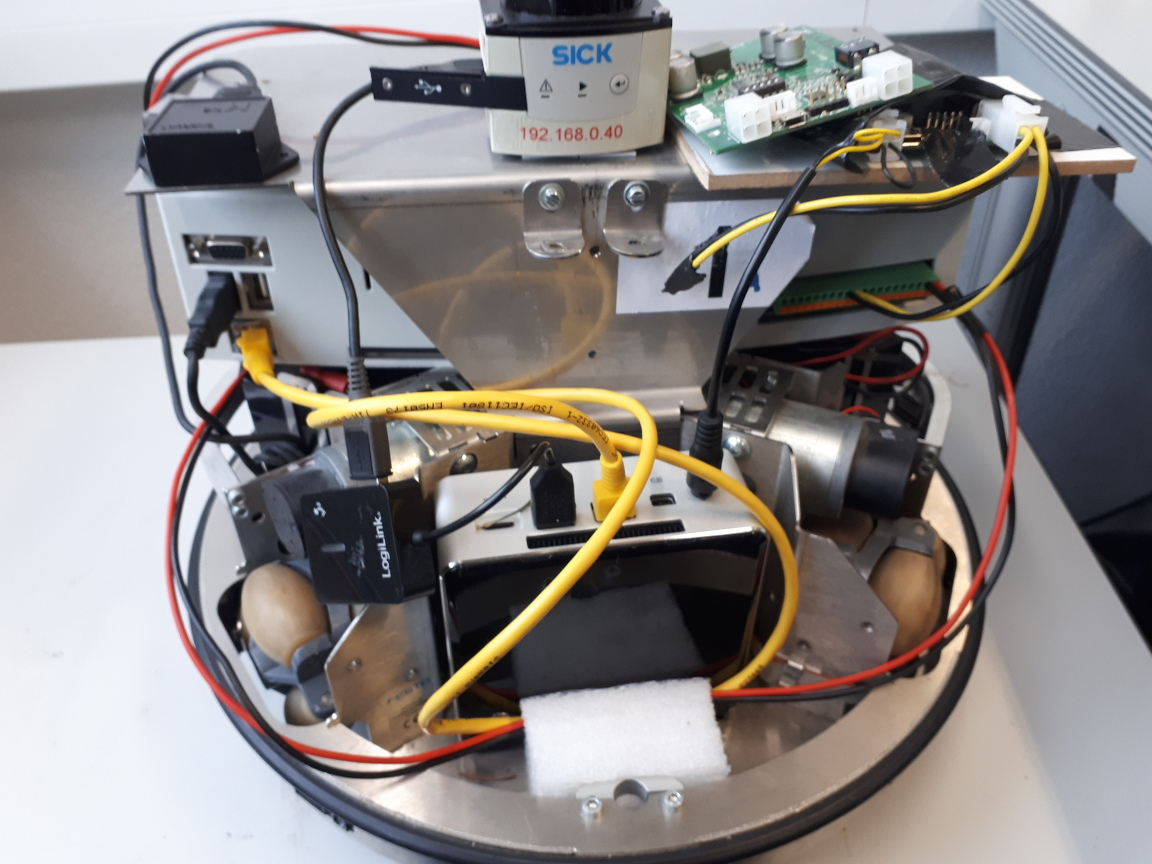
\includegraphics[width=0.5\textwidth]{robotino_front}
	\caption{[todo] Frontansicht des fertig aufgebauten Robotinos.}
	\label{fig:robotino_front}
\end{figure}


\begin{comment}
------------------------------------------------------------------------------------------
\end{comment}
\section{Softwarearchitektur [todo]}


\begin{comment}
------------------------------------------------------------------------------------------
\end{comment}
\subsection{ROS Module [todo]}


\begin{comment}
------------------------------------------------------------------------------------------
\end{comment}
\subsubsection{gmapping}

- This package contains a ROS wrapper for OpenSlam's Gmapping.
- The gmapping package provides laser-based SLAM (Simultaneous Localization and Mapping), as a ROS node called slam\_gmapping.
- Using slam\_gmapping, you can create a 2-D occupancy grid map from laser and pose data collected by a mobile robot.
\url{http://wiki.ros.org/gmapping}

Benötigt eine TF--Transformation zwischen base\_link und odom. Mittels der Odometry und dem Laser--Scans erzeugt er eine TF--Transformation zwischen map und odom.


\begin{comment}
------------------------------------------------------------------------------------------
\end{comment}
\subsubsection{hector\_trajectory\_server}

Mit diesem Modul ist es möglich die gefahrene Trajektorie eine Roboters in einem bestimmten Koordinatensystem auszugeben. Hierfür muss im TF--Tree eine Verbindung zwischen dem \textit{source\_frame\_name}(base\_link) und dem \textit{target\_frame\_name}(odom oder map) bestehen. Die Trajektorie bezieht sich mit ihren Koordinaten auf das target\_frame und ist vom Datentyp nav\_msgs/Path.

Über einen Service lässt die sich Trajektorie auch abfragen: \textit{rosservice call /trajectory}

\url{http://wiki.ros.org/hector_trajectory_server}

\url{http://docs.ros.org/api/nav_msgs/html/msg/Path.html}

\begin{listing}
	\begin{minted}[frame=single]{xml}
<node 
  name="hector_trajectory_server"
  pkg="hector_trajectory_server"
  type="hector_trajectory_server"
  output="screen">

  <param name="target_frame_name" value="map"/>
  <param name="source_frame_name" value="base_link" />
  <param name="trajectory_update_rate" value="10.0" />
  <param name="trajectory_publish_rate" value="10"/>
</node>
	\end{minted}
	\unskip
	\caption{Konfiguration der hector\_trajectory\_server--Nodes.}
	\label{lst:hector_trajectory_server_node}
\end{listing}


\begin{comment}
------------------------------------------------------------------------------------------
\end{comment}
\subsubsection{rf2o\_laser\_odometry}

\url{http://wiki.ros.org/rf2o}


\begin{comment}
------------------------------------------------------------------------------------------
\end{comment}
\subsubsection{robotino\_node}


\begin{comment}
------------------------------------------------------------------------------------------
\end{comment}
\subsubsection{robotino\_odometry\_node}

Sorgt dafür, dass die Odometry--Nachrichten vom Robotino ins ROS--System veröffentlicht werden.


\begin{comment}
------------------------------------------------------------------------------------------
\end{comment}
\subsubsection{Vergleich der Trajektorie von Odom und rf2o}

- Trajektorie der Robotino--Odometry bestimmen.
- Herausfiltern der Odometry Nachrichten aus den Bag--Dateien
- Odometry aus den Laser--Scans bestimmen und Trajektorie aufzeichen.
- Trajektorien vergleichen




\begin{comment}
------------------------------------------------------------------------------------------
\end{comment}
\subsection{MRPT Module [todo]}